\documentclass[a4paper,12pt,openany]{book}

% Paquetes básicos
\usepackage[utf8]{inputenc}   % Codificación de caracteres
\usepackage[T1]{fontenc}      % Codificación de fuentes
\usepackage[spanish]{babel}   % Idioma español

% Paquetes matemáticos
\usepackage{amsmath, amssymb} % Símbolos matemáticos

% Paquetes gráficos y tablas
\usepackage{graphicx}         % Inclusión de gráficos
\usepackage{booktabs}         % Tablas profesionales
\usepackage{multirow}         % Combinar celdas en tablas
\usepackage{makecell}         % Celdas personalizadas
\usepackage{colortbl}         % Colorear celdas específicas
\usepackage[table]{xcolor}    % Colores en tablas

% Paquetes para estilo y personalización
\usepackage{geometry}         % Configuración de márgenes
\usepackage{fancyhdr}         % Encabezados y pies de página
\usepackage{titlesec}         % Formato de títulos
\usepackage{caption}          % Personalización de leyendas
\usepackage{enumitem}         % Personalización de listas
\usepackage{tcolorbox}        % Cajas de color
\usepackage{float}            % Control de posición de figuras/tablas

% Paquetes de código y diagramas
\usepackage{tikz}             % Dibujos vectoriales
\usepackage{listings}         % Código fuente
\usepackage{color}            % Colores en código

% Paquetes adicionales
\usepackage{hyperref}         % Enlaces y referencias
\usepackage{eurosym}          % Símbolo del euro
\usepackage{pdfpages}         % Incluir PDFs
\usepackage{tocloft}          % Personalización de índice (TOC)

\usepackage{listings}
\lstset{
    basicstyle=\ttfamily\footnotesize,
    breaklines=true,
    frame=single
}


% Configuración de márgenes
\geometry{left=3cm, right=3cm, top=2.5cm, bottom=2.5cm}

% Configuración de encabezados y pies de página
\pagestyle{fancy}
\fancyhf{}
\fancyhead[L]{\nouppercase{Memoria Parcheckers}}
\fancyhead[R]{Inteligencia Artificial}
\fancyfoot[L]{\rule[0pt]{\textwidth}{0.2pt}\\}
\fancyfoot[C]{\rule[0pt]{\textwidth}{0.2pt}\\\thepage}
\fancyfoot[R]{\rule[0pt]{\textwidth}{0.2pt}\\}

\renewcommand{\sectionmark}[1]{\markboth{#1}{}} % Sección solo en encabezado izquierdo

% Formato de títulos
\titleformat{\section}{\large\bfseries}{\thesection.}{0.5em}{}
\titleformat{\subsection}{\normalsize\bfseries}{\thesubsection.}{0.5em}{}

% Personalización de índice (TOC)
\renewcommand{\cftchapfont}{\bfseries\large}
\renewcommand{\cftsecfont}{\mdseries}
\renewcommand{\cftsubsecfont}{\mdseries}
\renewcommand{\cftchappagefont}{\bfseries}
\renewcommand{\cfttoctitlefont}{\Huge\bfseries}
\renewcommand{\cftaftertoctitle}{\hfill} % Centra el título del índice
\setlength{\cftbeforechapskip}{1em}     % Espacio antes de capítulos
\setlength{\cftbeforesecskip}{0.3em}    % Espacio antes de secciones
\setlength{\cftbeforetoctitleskip}{1em} % Espacio antes del título del TOC
\setlength{\cftchapnumwidth}{3em}       % Ancho de números de capítulo
\setlength{\cftsecnumwidth}{4em}        % Ancho de números de sección

% Datos del documento
\title{\textbf{Memoria de Inteligencia Artificial Práctica 3 Parcheckers}}
\author{Ismael Sallami Moreno\\ \texttt{}}
\date{
  \vspace{1cm}
  \begin{tabular}{rl}
    \textbf{Asignatura:} & Inteligencia Artificial \\
    \textbf{Tema:} & Temario \\
    \textbf{Fecha:} & \today
  \end{tabular}
}

\begin{document}

% Portada
\begin{titlepage}
  \begin{center}
    \Huge \textbf{Memoria de Inteligencia Artificial Práctica 3: Parcheckers}
    \vspace{0.8cm}

    \begin{tikzpicture}[remember picture, overlay]
      \node[opacity=0.2] at (current page.center) {
\includegraphics[width=\paperwidth,height=\paperheight]{portada_parchis.png}};
      \node[align=center] at (current page.center) {
        \vspace{0.5cm}
        \LARGE \textbf{Ismael Sallami Moreno} \\
        \LARGE \texttt{} \\
        \LARGE \url{} \\
        \LARGE \url{} \\
        \vspace{2cm}
        \Large \textbf{Universidad de Granada}
      };
    \end{tikzpicture}
    \vfill
    \Large \textbf{2025}
  \end{center}
\end{titlepage}

\newpage

% Incluir licencia
%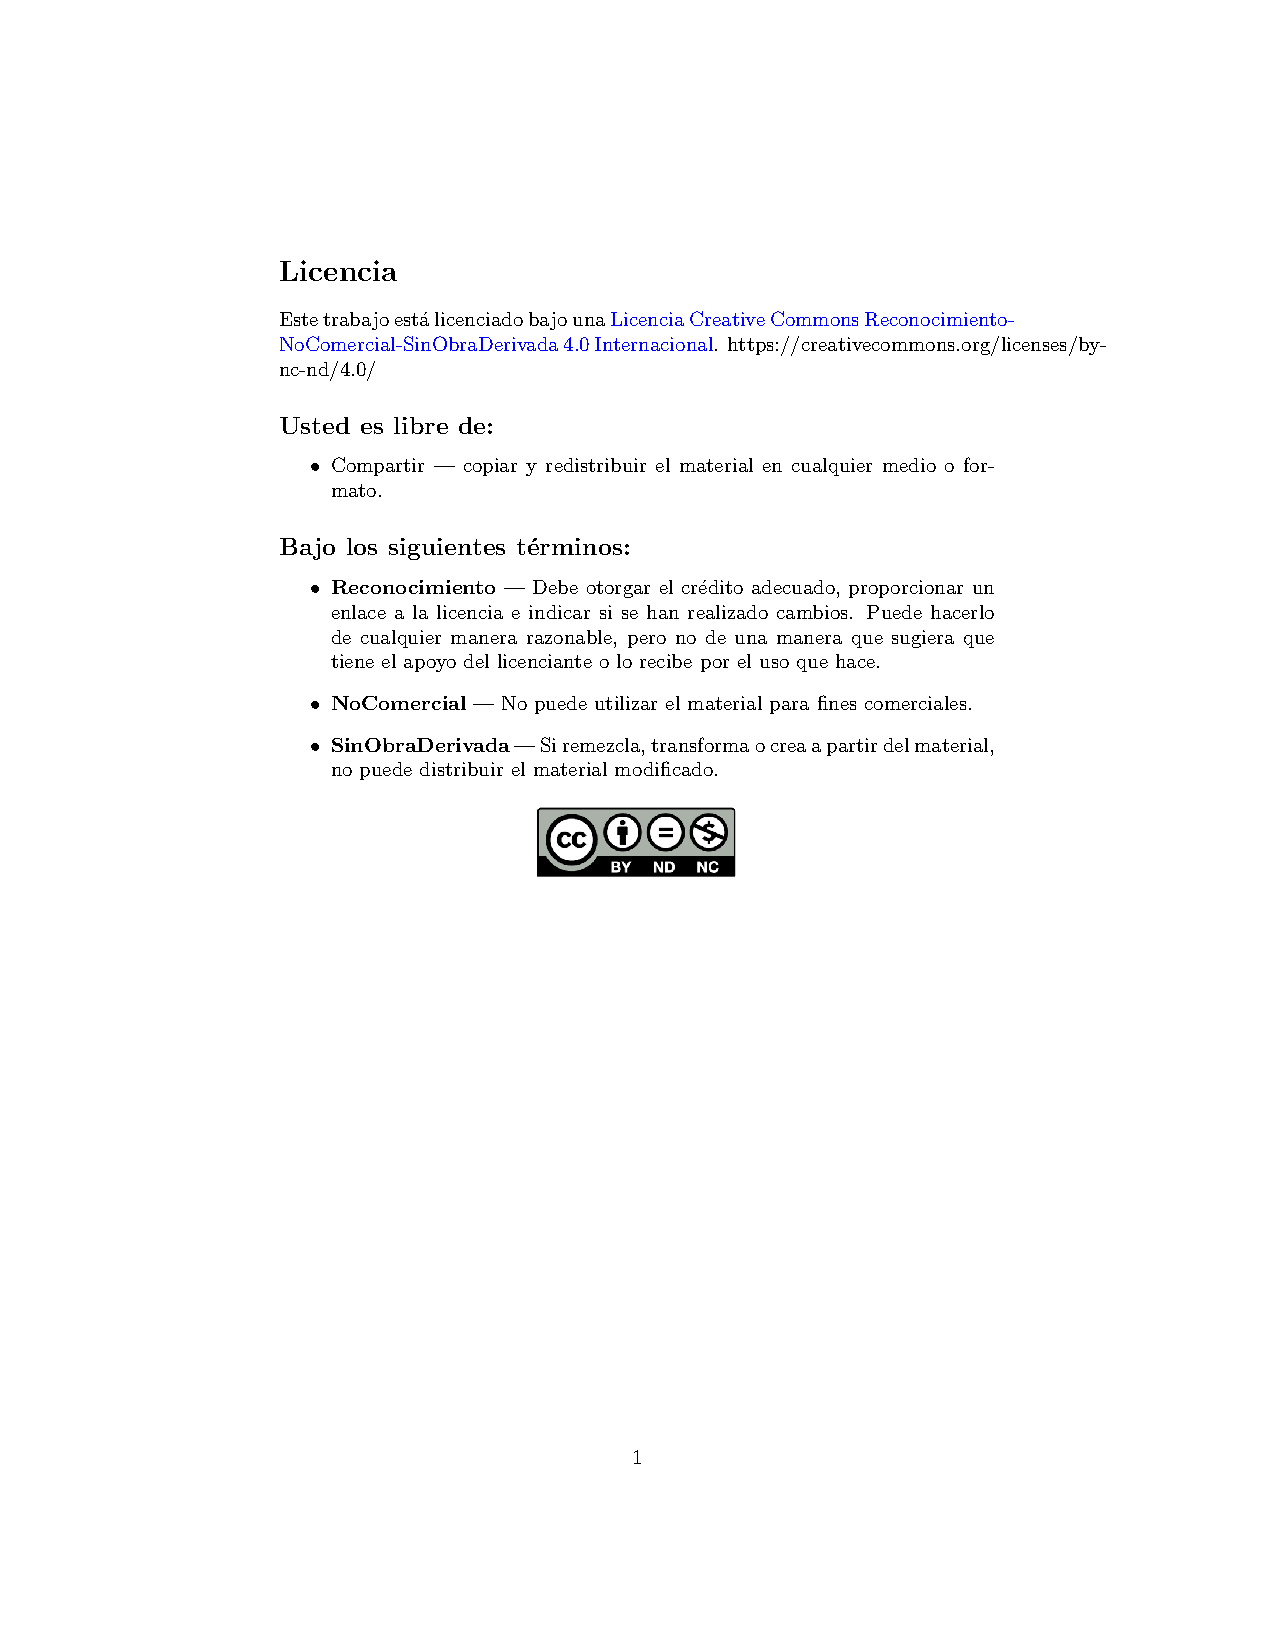
\includepdf[pages=-]{../../../../licencia.pdf}

% Índice de contenidos
\renewcommand{\contentsname}{\centering Índice General}
\tableofcontents
\newpage

\chapter*{Introducción}
\addcontentsline{toc}{chapter}{Introducción}
En esta práctica se ha trabajado en el desarrollo de un agente deliberativo para el juego \textit{ParCheckers}, una adaptación determinista del Parchís en la que cada jugador controla dos colores y puede elegir el dado a usar en cada turno. El objetivo principal ha sido implementar y mejorar el algoritmo de poda Alfa-Beta y distintas heurísticas, buscando un equilibrio entre la eficiencia computacional (límite de nodos generados y evaluados, así como un límite de tiempo por movimiento) y la calidad de las decisiones tomadas por el agente.

Se han desarrollado varias versiones del algoritmo de poda Alfa-Beta, incluyendo variantes con profundidad dinámica, ordenación de movimientos, poda probabilística y búsqueda de quietud. Cada versión ha sido diseñada con el propósito de mejorar la exploración del árbol de juego y aumentar las probabilidades de victoria frente a los adversarios controlados por inteligencia artificial (los ``ninjas''). \textit{Cabe destacar que aunque el código parece estar correcto, el hecho de que se venza o no a los ninjas depende de la implementación de la heurística.}

Asimismo, se han creado distintas heurísticas que permiten valorar los estados del juego en función de criterios como la distancia a la meta, la seguridad de las fichas y las barreras, con el fin de dotar al agente de una estrategia más competitiva. Todas estas implementaciones han sido evaluadas y comparadas en un conjunto de partidas contra los jugadores automáticos del simulador, así como enfrentando heurísticas entre sí como se aconseja en el guión, con el objetivo de analizar su rendimiento y justificar las decisiones tomadas a lo largo del proceso.

\textit{Cabe destacar que me hubiese gustado poder dedicar más tiempo a esta práctica, ya que he aprendido mucho, pero al estar en época de exámenes y demás no he podido dedicarle el tiempo necesario.} Por otro lado, he priorizado el aprender los algoritmos de manera correcta\footnote{Se puede apreciar en el código numerosas implementaciones.}, para ello me he basado en libros y otros recursos.

Se añade la bibliografía de los libros y/o artículos que se han utilizado para la búsqueda de algoritmos, además de diversas fuentes de Internet que se han consultado para la implementación de las distintas heurísticas y el algoritmo de poda Alfa-Beta y demás herramientas (algún simulador de algoritmos de búsqueda, video de YouTube, etc.)\footnote{Estos últimos no se incluyen porque creo que son irrelevantes, solo se incluyen los libros.}.
\chapter*{Descripciones detalladas de las versiones de poda}
\addcontentsline{toc}{chapter}{Descripciones detalladas de las versiones de poda}

\section*{Poda Alfa-Beta Clásica}
La poda Alfa-Beta clásica es la optimización fundamental del algoritmo Minimax, que utiliza dos cotas, $\alpha$ y $\beta$, para evitar expandir ramas que no pueden alterar la decisión final. $\alpha$ representa la mejor puntuación que puede garantizar el jugador MAX hasta ese momento, mientras que $\beta$ es la mejor puntuación que MIN puede asegurar. Si en algún punto $\alpha \geq \beta$, la rama puede ser descartada de forma segura, ya que no aportará ninguna mejora al resultado global. Esta técnica reduce drásticamente el número de nodos explorados en comparación con el Minimax puro. En este contexto se debe tener en cuenta de no sobrepasar el límite de nodos generados y evaluados, así como el límite de tiempo por movimiento, para garantizar un rendimiento óptimo del agente.

\section*{Poda Alfa-Beta Ordenada}
En esta variante, se incorpora un paso previo de ordenación de los hijos antes de expandirlos. Concretamente, los nodos hijos se ordenan utilizando la heurística (de forma descendente en MAX y ascendente en MIN). La razón de esta mejora es que, si se examinan primero los movimientos más prometedores, las cotas $\alpha$ y $\beta$ se actualizan antes y permiten podar más ramas en niveles superiores, acelerando significativamente la búsqueda. Para su implementación, se utiliza una función de ordenación que prioriza los nodos con mayor puntuación heurística, lo que mejora la eficiencia del algoritmo al reducir el número de nodos explorados. Al ordenarse en base a la heurística, el orden depende fundamentalmente de la calidad de la heurística utilizada, por ende, si la heurística no es del todo correcta y el algoritmo es perfecto, no se va a obtener el resultado esperado (óptimo).

\section*{Poda Alfa-Beta Probabilística}
Esta versión introduce un parámetro de tolerancia $\epsilon$ que relaja el criterio clásico de poda. En lugar de podar sólo cuando $\alpha \geq \beta$, se permite la poda anticipada si la diferencia $\beta - \alpha$ es menor que $\epsilon$. Con esto se asume que es poco probable que la rama mejore significativamente el resultado, y se corta la exploración para ganar velocidad a cambio de una ligera pérdida potencial de calidad en la jugada elegida. Es una técnica especialmente útil para profundizar más sin comprometer demasiado el rendimiento general. La implementación se ha basado fundamentalmente en lo mencionado, si la rama no es ``bastante prometedora'', se poda. Cabe destacar que he optado por un valor de $\epsilon$ de 0.3, el cual es bastante pequeño, pero es que tras numerosas pruebas era el valor que mejor se ajustaba\footnote{También se realizaron pruebas con 0,5 y 0 para ver si con solo la poda alfa-beta y quietud bastaba, pero los resultados eran bastante peores.}.

\section*{Profundidad Dinámica}
La profundidad dinámica adapta la profundidad máxima de búsqueda en función de la cantidad de hijos generados en un nodo. La idea es que, cuando hay pocas opciones (baja ramificación), se puede profundizar más para explorar jugadas con mayor precisión. Por el contrario, cuando hay muchas opciones (alta ramificación), se limita la profundidad para no sobrepasar el número máximo de nodos. Así, se equilibra la carga de cómputo y se aprovechan mejor los recursos disponibles. En este punto pensé en ampliar la profundidad máxima de búsqueda, pero había casos en los que si podía entrar en esa rama y tardar una infinidad de tiempo.

\section*{Búsqueda de Quietud}
La búsqueda de quietud se utiliza para evitar evaluaciones engañosas en estados de juego inestables. Cuando se alcanza la profundidad máxima y el estado no es "quiescente" (hay capturas o movimientos tácticos relevantes inminentes), se siguen explorando exclusivamente esas jugadas tácticas. Así se obtiene una evaluación más realista del estado final. Esto ayuda a mitigar el efecto de los ``horizontes artificiales'' que pueden inducir decisiones erróneas en situaciones críticas.
La lógica comienza evaluando el estado actual como \texttt{stand\_pat\_score}. Si no hay movimientos tácticos, devuelve ese valor directamente. Si los hay, explora recursivamente solo esos hijos tácticos, actualizando los valores \texttt{alpha} o \texttt{beta} y aplicando poda cuando corresponde (\texttt{beta <= alpha}). De esta forma, permite “dejar que se resuelva el caos” antes de tomar decisiones finales, evitando evaluaciones erróneas por cambios bruscos en la posición. Esta búsqueda se detiene cuando se alcanza la profundidad máxima de quietud o se llega a un estado estable.

\section*{Versión Combinada: Poda Alfa-Beta Ordenada, Probabilística y Dinámica}
La versión más avanzada que hemos implementado combina varias de las mejoras anteriores en un único algoritmo. Integra:
\begin{itemize}
    \item La ordenación de los hijos para podar más rápidamente.
    \item La poda probabilística para cortar ramas menos prometedoras de forma anticipada.
    \item El ajuste dinámico de la profundidad según la ramificación del árbol.
    \item Además, utiliza la búsqueda de quietud en los nodos límite para evitar evaluaciones precipitadas.
\end{itemize}
Este enfoque integral permite un equilibrio óptimo entre la calidad de las decisiones y el tiempo de respuesta, maximizando la competitividad del agente frente a adversarios exigentes.
Aunque desde el punto de vista teórico, se ve que funciona correctamente, tras numerosas pruebas, nuestra heurística funcionaba de mejor manera en la implementación del algoritmo de poda alfa-beta probabilística y quietud con un valor de $\epsilon$ de 0.3, es decir, casi despreciable, y con ayuda de la búsqueda de quietud. Gracias a esto se ha logrado vencer $4/6$ casos posibles (3 ninjas, teniendo en cuenta los casos en los que puedo empezar yo o el ninja). \textit{Curiosamente se llego a la conclusión de que en mi caso, y repito, tras numerosas pruebas de heurísticas y valores de las mismas, se podía adoptar ``un cambio dinámico de los valores de la heurística'', lo que se traduce en que si empiezo yo (el id es 0) adopto unos valores determinados y si empieza el ninja (el id es 1) adopto otros valores. Pero esto no se ha implementado debido a que no es lo que se pedía en el enunciado.} 



\chapter*{Búsqueda de Quietud: Motivación y Explicación}
\addcontentsline{toc}{chapter}{Búsqueda de Quietud: Motivación y Explicación}

La búsqueda de quietud es una técnica que se añade a los algoritmos de poda para evitar que la evaluación final se base en estados tácticamente inestables. Al llegar a la profundidad máxima, en muchos casos el algoritmo podría detenerse justo antes de jugadas clave (por ejemplo, capturas o creación de barreras). Si se evaluara directamente ese estado, la puntuación sería engañosa, porque no refleja la verdadera seguridad o ventaja que tendría el agente en el turno siguiente.

Por eso, la búsqueda de quietud permite seguir explorando \emph{únicamente} las ramas tácticamente relevantes (movimientos de comer ficha, de llegar a meta, etc.) hasta que la posición resultante sea ``tranquila''. Esto asegura una evaluación más realista y menos afectada por el llamado \emph{horizonte} de búsqueda.

El umbral \texttt{UMBRAL\_DELTA} se emplea para decidir qué diferencia de heurística es lo bastante importante como para seguir explorando. Si la diferencia entre un hijo y su padre es mayor a ese umbral, el nodo no se considera quieto y se siguen explorando movimientos tácticos.

La función \texttt{BusquedaQuietud} está diseñada para ampliar la búsqueda en aquellas situaciones donde la evaluación directa del estado podría resultar engañosa debido a movimientos tácticos inminentes. En su inicio, la función comprueba si se ha alcanzado el límite de nodos permitido (\texttt{NodeCounter}) o la profundidad máxima establecida para la búsqueda de quietud. Si se cumple cualquiera de estas condiciones, se devuelve directamente la evaluación heurística del estado actual (almacenada en la variable \texttt{stand\_pat\_score}).

A continuación, se ajustan las cotas \texttt{alpha} y \texttt{beta} en función de si el nodo actual es de tipo MAX o MIN, siguiendo la lógica clásica de poda Alfa-Beta. Después, se generan los hijos del estado actual, pero se filtran solo aquellos que correspondan a movimientos tácticos relevantes, como comer una ficha o llegar a meta. Este filtrado es fundamental para enfocar la búsqueda en aquellas jugadas que pueden cambiar sustancialmente la evaluación del estado y garantizar que no se ignoren situaciones clave.

Si no se encuentran movimientos tácticos, significa que el estado es estable (quieto) y la función devuelve la evaluación directa del estado actual. Sin embargo, si hay movimientos tácticos disponibles, estos se exploran recursivamente, actualizando las cotas \texttt{alpha} y \texttt{beta} y aplicando la poda correspondiente cuando es necesario. La exploración se detiene en cuanto se cumple la condición de poda.

En definitiva, esta implementación permite refinar la evaluación de los estados ``no estables'' de forma eficiente, integrándose con la poda Alfa-Beta y enfocándose en los movimientos más significativos para la dinámica de la partida.



\vspace{1em}

\chapter*{Resumen de las Heurísticas y Elección de la Mejorada}
\addcontentsline{toc}{chapter}{Resumen de las Heurísticas y Elección de la Mejorada}

A lo largo de esta práctica se han explorado y probado diversas heurísticas para evaluar la calidad de un estado del juego de \emph{Parcheckers}. Las primeras versiones (partiendo de la heurística ValoracionTest que se nos ofrece), como \texttt{Heur1} y \texttt{Heur2}, se enfocaban en aspectos básicos como la distancia de las fichas a la meta, la seguridad de las casillas ocupadas y la presencia de barreras propias o enemigas. Estas heurísticas resultaron útiles para obtener una visión general del estado del tablero y para equilibrar el progreso ofensivo y la seguridad defensiva. Esta parte se va intentar hacer lo más breve posible, ya que se han implementado numerosas heurísticas, similares entre sí, pero a la vez diferentes. Se optó por el desarrollo de la heurística PruebaH, mas simple que Heur1 y Heur2, debido a que ofrecía mejores resultados usando la Poda Alfa-Beta.

A continuación, se desarrollaron otras variantes como la \texttt{HeuristicaNueva}, que añadía ponderaciones diferenciadas para las distancias y la cantidad de fichas en meta o seguras. Finalmente, se diseñó la \textbf{Heurística Mejorada}, que combina los elementos esenciales de las versiones anteriores y añade una lógica más elaborada para ponderar la vulnerabilidad de las propias fichas y la amenaza que representan las fichas del oponente. De igual manera reducí la complejidad del algoritmo y me quede con lo esencial ajustando los pesos y esta vez usando el algoritmo de poda Alfa-Beta Probabilística y quietud conseguí el mejor resultado posible. 

% Las lógicas de las heurísticas han sido:
% \begin{itemize}
%     \item La lógica implementada en la \texttt{Heurística Mejorada} se basa en calcular dos puntuaciones separadas: una para el jugador IA y otra para el oponente. Se valoran de forma positiva los factores como la cercanía a la meta, las fichas en meta, la seguridad de las casillas, y la formación de barreras. Por otro lado, se penalizan los factores como la presencia de fichas en casa o la vulnerabilidad a capturas. Esta evaluación diferencial permite capturar no sólo el estado posicional propio, sino también las amenazas que suponen las fichas del adversario.
% \end{itemize}

\section*{Lógicas de las Heurísticas}
Las lógicas de las heurísticas han sido:

\begin{itemize}
    \item La \texttt{Heur1} pondera factores como la distancia a la meta (priorizando el progreso), la seguridad de las fichas (casillas seguras) y la formación de barreras propias o rivales. Se suman las puntuaciones de las fichas propias y se restan las del oponente, obteniendo un diferencial que refleja la situación general del tablero.
    
    \item La \texttt{Heur2} amplía la anterior incorporando un conteo más detallado de barreras (mediante un mapa de casillas ocupadas) y una penalización o bonificación en función del total de barreras del oponente y propias. Además, incluye un término que compara la mínima distancia a meta del oponente con la de las fichas propias, ponderando la ventaja táctica en el avance relativo.
    
    % \item La \texttt{PruebaH} simplifica la evaluación priorizando únicamente la distancia a la meta y el tipo de casilla donde se encuentran las fichas (por ejemplo, dando bonificaciones a las que están en la meta o en la fila final). Aunque es menos rica en matices que las anteriores, es muy ligera computacionalmente y permite un cálculo rápido y directo de la puntuación diferencial entre el jugador y el oponente, ofreciéndome mejores resultados.

    \item La \texttt{PruebaH} mantiene una lógica relativamente sencilla pero con varias mejoras clave. Calcula la puntuación sumando la cercanía a la meta (distancia normalizada), la presencia en casillas de meta, la seguridad (fichas en casillas seguras) y la bonificación por estar en la fila final (\texttt{final\_queue}). Penaliza, por otro lado, las fichas que están en casa (\texttt{home}). Esta evaluación se realiza tanto para las fichas del jugador como para las del oponente, obteniendo la puntuación final como la diferencia entre ambos. Esta heurística está diseñada para capturar de forma rápida los aspectos esenciales del progreso y la seguridad, manteniendo un cómputo ligero y eficiente. \textbf{Tras numerosas pruebas, me di cuenta que lo mas importante de la heurística era la asignación de pesos.}
    
    \item La \texttt{HeuristicaNueva} se centra en un modelo más simplificado: pondera directamente la distancia a meta (con un peso negativo para representar que menor distancia es mejor), el número de fichas en meta y la seguridad de las piezas. Añade bonificaciones específicas si hay capturas o si se llega a la meta en el último movimiento. Su lógica es más directa y fácil de ajustar, pero menos rica en matices que las anteriores.
    
    \item La \texttt{Heurística Mejorada} combina elementos de las anteriores, calculando dos puntuaciones separadas: una para el jugador IA y otra para el oponente. Se valoran positivamente la cercanía a la meta, la seguridad de las casillas ocupadas y la formación de barreras, mientras que se penaliza la presencia de fichas en casa y la vulnerabilidad a capturas. Esta evaluación diferencial permite capturar no solo la situación de progreso propio, sino también la amenaza y la posición de las fichas rivales.
\end{itemize}


Tras comparar los resultados prácticos de las distintas heurísticas, se decidió mantener la \textbf{Heurística Mejorada} como la opción principal. Esto se debe a que ofrece un equilibrio consistente entre agresividad y defensa, incorporando tanto la dinámica de progreso hacia la meta como la protección de las fichas, y proporcionando una evaluación más completa de las posiciones de juego. Gracias a este enfoque, el agente logra tomar decisiones más inteligentes y adaptativas en las partidas, superando a otras variantes en la mayoría de los escenarios probados. Cabe destacar que aunque en el guión se menciona las funciones \textit{distanceToGoal} y \textit{distancetoBox}, estas se han usado de la manera que mejor resultado me han ofrecido.



    
    
    

\chapter*{Podas Implementadas y Selección Final}
\addcontentsline{toc}{chapter}{Podas Implementadas y Selección Final}

Durante el desarrollo del agente se han implementado varias variantes de poda para optimizar el proceso de búsqueda y toma de decisiones en el juego. Entre ellas destacan la poda \textbf{Alfa-Beta clásica}, que sirve como base para comparar el resto de mejoras, la \textbf{Poda Alfa-Beta Ordenada}, que ordena los nodos antes de explorar para mejorar la eficiencia, y la \textbf{Poda Alfa-Beta Probabilística}, que introduce un factor de probabilidad (epsilon\_prune) para permitir cortes anticipados cuando las diferencias entre alpha y beta son poco significativas.

Además, se implementó la versión más avanzada conocida como \textbf{Poda Alfa-Beta Probabilística Ordenada y Dinámica}, que combina la ordenación de hijos con la adaptación dinámica de la profundidad máxima según la ramificación y el contexto del juego. Aunque esta última es conceptualmente la más robusta y, en teoría, la más potente en términos de rendimiento y precisión, en las pruebas prácticas no siempre ofrecía ventajas claras sobre el resto.

Finalmente, la elección para la versión final del agente fue la \textbf{Poda Alfa-Beta Probabilística} (con parámetro de epsilon), ya que ofrecía un excelente equilibrio entre eficiencia y simplicidad, especialmente al integrarse con la \emph{Heurística Mejorada} y el uso de la \textit{Búsqueda de Quietud}. En las comparativas internas, esta combinación demostró superar de forma consistente a las versiones más avanzadas, tanto en tiempo de respuesta como en la solidez de las decisiones tomadas. La simplicidad de su lógica también facilita la depuración y el mantenimiento del código, haciendo de esta poda la opción final para el agente entregado.

Se cumple con los requisitos del guión ya que se ha optado por una poda alfa beta, probabilística e implentando quietud (3/5 mejoras), aunque en la práctica no haya dado mejores resultados la versión combinada de poda Alfa-Beta Ordenada, Probabilística y Dinámica, que se suponía que debía de darlos al ser más completa.

\chapter*{Mejora Extra Propuesta: Ajuste Dinámico de Pesos Heurísticos}
\addcontentsline{toc}{chapter}{Mejora Propuesta: Ajuste Dinámico de Pesos Heurísticos}

Como propuesta adicional para mejorar el rendimiento del agente\footnote{En el guión se menciona que se pueden aportar ideas extras valorándose la eficiencia y demás.}, se ha implementado una funcionalidad que adapta dinámicamente los pesos de la heurística en función de la fase de la partida. La idea central es que, a medida que la partida avanza y las condiciones del tablero cambian, los criterios para decidir qué movimientos son mejores también varían.

Para ello, se ha diseñado una función \texttt{ajustarPesosSegunFaseDePartida()} que analiza el número total de fichas en meta (tanto propias como del oponente) y clasifica la partida en tres fases:

\begin{itemize}
    \item \textbf{Fase inicial (pocas fichas en meta):} se da prioridad al avance rápido y la movilidad, disminuyendo la penalización por vulnerabilidad.
    \item \textbf{Fase intermedia (varias fichas en meta):} se busca un equilibrio entre progreso, seguridad y defensa.
    \item \textbf{Fase final (muchas fichas en meta):} se refuerza la prioridad de llevar fichas a meta y se penaliza más la vulnerabilidad.
\end{itemize}

De este modo, la IA adapta su comportamiento y sus prioridades a la situación de la partida, logrando una mayor flexibilidad y competitividad frente a diferentes rivales y estilos de juego. Aunque esta mejora no estaba contemplada en el enunciado, su integración ha demostrado un impacto positivo en la estabilidad y la capacidad del agente para adaptarse, superando en algunos casos a la heurística estática y contribuyendo a la obtención de mejores resultados frente a los ninjas. En el código se ha decidido comentarlo debido a que produce el mismo mejor resultado, pero con casos distintos.


\chapter*{Comparaciones de Heurísticas y Algoritmos}
\addcontentsline{toc}{chapter}{Comparaciones de Heurísticas y Algoritmos}

A continuación, se introduce una tabla\footnote{Como se especifica en el guión, se ha añadido una tabla con las distintas heurísticas y sus puntuaciones, he considerado las más relevantes, las otras las he dejado en el código para que el profesor pueda verlas.} comparando las heurísticas implementadas, sus puntuaciones y el porque del resultado obtenido\footnote{Se hace referencia a n/p con $p_{max} = 6$ debido a que se tiene en cuenta que son 3 ninjas y que puede empezar o él o yo. }:


\begin{table}[H]
    \centering
    \renewcommand{\arraystretch}{1.2} % Aumenta ligeramente el espacio entre filas
    \resizebox{\textwidth}{!}{ % Ajusta la tabla al ancho de la página
    \begin{tabular}{|p{3.5cm}|p{2.2cm}|p{4cm}|p{6cm}|p{1cm}|} % Añadido el | al final
    \hline
    \textbf{Heurística} & \textbf{Puntuación} & \textbf{Algoritmo} & \textbf{Explicación} & \textbf{ID} \\
    \hline
    PruebaH & 3/6 & Poda Alfa Beta & Resultado esperado: un algoritmo simple con una heurística simple también vence a más ninjas que la heurística mejorada (comparo distancias hacia la meta y demás). & 3 \\
    \hline
    Heurística Mejorada & 4/6 & Poda Alfa Beta, Probabilística y Quietud & Es el mejor resultado entre los algoritmos presentes. Con un $\epsilon$ bajo se evita descartar caminos prometedores, y la heurística (centrada en la distancia a las fichas de casa y un manejo simple de las barreras) funciona mejor. & 1 \\
    \hline
    Heurística Mejorada & 1/6 & Poda Alfa Beta, Probabilística, Ordenada, Dinámica y usando Quietud & Al intentar introducir tantas mejoras, la carga del algoritmo es demasiado alta, lo que aumenta el tiempo de respuesta. El resultado es bajo porque la heurística no encaja del todo: habría que mejorar el tratamiento con las barreras o la distancia a la meta, o bien asignar pesos dinámicos según la fase de la partida. & 2 \\
    \hline
    \end{tabular}
    }
    \caption{Comparativa de heurísticas implementadas.}
    \label{tab:heuristicas_comparativa}
\end{table}

    
No añado los demás casos porque no son relevantes, ya que se han implementado numerosas heurísticas y pruebas de algoritmos, pero he decidido incluir los más importantes. Adjunto imagen de los intentos con el bot para aportar más información al profesor(añado solo la parte final):

\begin{figure}[H]
    \centering
    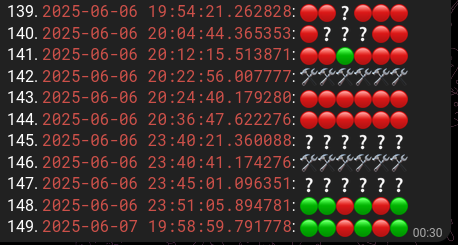
\includegraphics[width=0.5\textwidth]{images/memoria.png}
    \caption{Resultados de las partidas con las distintas heurísticas.}
    \label{fig:partidas_resultados}
\end{figure}



\input{Capitulos/Conclusion_memoria.tex}
% \chapter*{Memoria de Prácticas}
\addcontentsline{toc}{chapter}{Memoria de Prácticas}

\section*{1. Mejoras de la Poda Alfa-Beta}
A lo largo del desarrollo de la práctica se han implementado varias versiones del algoritmo de poda Alfa-Beta, buscando mejorar la eficiencia y precisión de la búsqueda. Las principales mejoras son:

\begin{itemize}
    \item \textbf{Poda Alfa-Beta Clásica:} La versión básica del algoritmo, que utiliza los límites $\alpha$ y $\beta$ para descartar ramas que no afectan la decisión final.
    \item \textbf{Poda Alfa-Beta Ordenada:} Añade un paso previo de ordenación de los hijos según la heurística. Así, los mejores nodos se exploran primero, incrementando las podas y reduciendo el número de nodos visitados.
    \item \textbf{Poda Alfa-Beta Probabilística:} Incorpora un parámetro $\epsilon$ que permite cortar ramas con diferencias mínimas entre $\alpha$ y $\beta$, priorizando la velocidad a costa de una ligera pérdida de precisión.
    \item \textbf{Profundidad Dinámica:} Ajusta la profundidad de búsqueda según la ramificación. Con menor ramificación, se profundiza más; con mayor ramificación, se limita para no exceder el número máximo de nodos.
    \item \textbf{Búsqueda de Quietud:} Extiende la exploración en situaciones tácticas inestables (capturas, barreras) para evitar evaluaciones engañosas en estados “no quietos”.
\end{itemize}

La combinación de estas mejoras permite un equilibrio entre calidad de las decisiones y tiempo de respuesta.

\section*{2. Heurísticas Propuestas}
Se han diseñado varias heurísticas para evaluar la calidad de los estados de juego, destacando:

\begin{itemize}
    \item \textbf{Heur1 y Heur2:} Primeras versiones, basadas en la distancia a la meta y la seguridad de las casillas.
    \item \textbf{HeuristicaNueva:} Añade ponderaciones diferenciadas para las distancias y la seguridad de las fichas.
    \item \textbf{Heurística Mejorada:} Combina los elementos anteriores y añade lógica para ponderar la vulnerabilidad de las fichas propias y la amenaza de las del oponente.
\end{itemize}

\section*{3. Tabla Comparativa}
A continuación, se incluye una tabla comparativa de las heurísticas implementadas, sus puntuaciones y el algoritmo de poda utilizado:

\begin{table}[H]
    \centering
    \renewcommand{\arraystretch}{1.2}
    \resizebox{\textwidth}{!}{
    \begin{tabular}{|p{3.5cm}|p{1.5cm}|p{4cm}|p{6cm}|}
    \hline
    \textbf{Heurística} & \textbf{Puntuación} & \textbf{Algoritmo} & \textbf{Explicación} \\
    \hline
    Heuristica Mejorada & 1/6 & Poda Alfa Beta, Probabilística, Ordenada, Dinámica y usando Quietud & La carga del algoritmo es demasiado alta, lo que aumenta el tiempo de respuesta. El resultado es bajo porque la heurística no encaja del todo. \\
    \hline
    PruebaH & 3/6 & Poda Alfa Beta & Algoritmo simple con heurística simple que vence a más ninjas que la heurística mejorada. \\
    \hline
    Heurística Mejorada & 4/6 & Poda Alfa Beta, Probabilística y Quietud & Es el mejor resultado. Con un $\epsilon$ bajo se evitan caminos poco prometedores y la heurística funciona mejor. \\
    \hline
    \end{tabular}
    }
    \caption{Comparativa de heurísticas implementadas.}
    \label{tab:heuristicas_comparativa}
\end{table}

\section*{4. Análisis de los Resultados}
Las diferentes versiones de la poda han permitido mejorar progresivamente la eficiencia y la precisión de la IA. Las primeras versiones ofrecían resultados limitados, mientras que la combinación de poda probabilística y búsqueda de quietud ha demostrado un equilibrio óptimo entre calidad y velocidad de respuesta.

Aunque la versión más completa (ordenada, probabilística y dinámica) parecía teóricamente la más sólida, en las pruebas reales no ofreció mejoras claras frente a la versión probabilística con quietud y un $\epsilon$ bajo.

\section*{5. Reflexión Personal}
Durante el desarrollo, se enfrentaron dificultades para equilibrar la calidad de la heurística con el tiempo de respuesta del algoritmo, especialmente en las versiones más avanzadas con ramificación dinámica. Fue especialmente interesante observar cómo pequeños cambios en la heurística podían tener un gran impacto en el rendimiento global del agente, obligando a realizar numerosas pruebas y ajustes para lograr la mejor configuración.



% Ejemplo de capítulos y secciones
% \chapter{Introducción}
% \section{Apuntes de clase}
% \section{Introducción: Inteligente}
Debemos de definir la inteligencia artificial
usando la palabra inteligente, la cual es difícil de definir. Se dan diferentes definiciones de Harvard y otras universidades/entidades reconocidas. 

\section{Definición de IA}

Podemos tener varias definiciones de IA, como pueden ser sistemas que actúan/piensan como humanos, o bien sistemas que actúan/piensas racionalmente. Una de ellas puede ser: "Campo de estudio que busca explicar y emular el comportamiento inteligente en términos de procesos computacionales"

Un ejemplo de IA que menciona el profesor reiteradamente es el caso de los \textit{cajeros automáticos}.

\begin{tcolorbox}[colback=blue!20, colframe=blue]
Se garantiza que una pregunta sobre las definiciones de IA cae.
    
\end{tcolorbox}

Asociamos el concepto de IA a racional debido a que se quiere desarrollar con la capacidad de poder tomar decisiones como los humanos.

Hay distintos softwares en los dispositivos que podemos relacionarlos con la acción de que \textit{piensan} debido a que usan inteligencia artifical, como es el caso de programas de ajedrez. ¿Es esto correcto? No podemos afirmar esto exactamente, ya que según autores pensar es emular la mente humana, cosa que no es capaz de hacer la IA debido a que solo esta entrenado a hacer las mejores jugadas para ganarte, mientras que tu puedes pensar sobre otras temáticas y tener cierto \textit{pensamiento libre}.

Si afirmamos que piensan como humanos, debemos de tener en cuenta el \textit{pensamiento cognitivo}.

La IA según el libro del \textit{Porque} (recibió el premio Turing), tiene 3 niveles:
\begin{enumerate}
    \item Aprendizaje automático.
    \item Simular al humano.
    \item Capacidad de imaginar, lo cual, a día de hoy es inalcanzable.
\end{enumerate}

En cuanto a la creatividad, hay cierta\textit{ creatividad cognitiva }en temas específicos.

El llamado 'no alineamiento con los humanos' es lo que ocurre cuando una IA no tiene información sobre ese tema o bien no esta entrenado, pues en este caso se lo inventa.

El Test de Turing, es aquel en el que si una IA consigue pasar desapercibido como humano, pues efectivamente pasa este Test.

En esta asignatura vamos a seguir la Teoría del Agente, que es la idea más aceptada hoy día y más usada. Este percibe el entorno y actúa de una manera específica. 

Se usa la palabra \textit{racional} aludiendo a inteligente.

Un agente racional actúa de manera correcta según la información que posee.

El origen del término de IA recae en John McCarthy. Los pioneros de la IA son varios, entre los que podemos encontrar a Alan Turing, Marvin Minsky,...

En el debate de la IA se menciona una IA fuerte y una débil, que son sistemas que actúan como humanos y racionalmente vs las que piensan como IA.

En cuanto al recorrido de la IA a lo largo de la historia, podemos destacar distintas épocas como es la Edad de Oro, Invierno de IA,...

Von Neumann propone el algoritmo MiniMax, el que afirma que el juego es una situación conflictiva en la que tomamos decisiones sabiendo que los demás también las toman, determinando el resultado en base a las decisiones realizadas.
Un hecho histórico destacable, es que Napoleón murió pensando que había perdido jugando al ajedrez pensando que perdió frente al primer sistema inteligente, aunque puede que haya sido un humano. 
Otro de los avances importantes es el caso de los cohes autónomos.

En cuanto a los tipos de IA podemos mencionar:

\begin{itemize}
    \item IA débil: una máquina que compite con un humano en una actividad específica.
    \item IA fuerte: IA que aplica inteligencia para cualquier problema.
    \item IA general: alcanza el nivel cognitivo humano.
    \item Super-IA: capacidad que es mucho mayor que cualquier cerebro humano en cualquier campo.
\end{itemize}

% \chapter{Agentes}
% \section{Concepto}
La Teoría de Agentes(denotado a continuación como \textbf{TA}) es un sistema de ordenador, situado en un entorno, capaz de realizar acciones de manera autónoma y que es flexible en base a las situaciones que se le presentan.

\section{Agentes Inteligentes}

Desarrolla un enfoque basado en agentes y lleva a cabo percepciones procesada mediante algoritmos de análisis y toma de decisiones. 
La TA se usa actualmente en la mayoría de ámbitos y es lo que más se usa hoy en día.

En cuanto a los tipos de agentes encontramos:

\begin{itemize}
    \item Reactivo: reacciona en base al entorno.
    \item Pro-activo: no solo actúan en respuesta al entorno, sino que puedan analizar acciones a llevar a cabo.
    \item  Social: son además capaces de interactuar.
    \item Multiagente: esta implementado como varios agentes interactuando.
\end{itemize}

La interacción entre agentes se lleva a cabo mediante: cooperación, coordinación y la negociación.


\section{Arquitecturas de Agentes}

Podemos distinguir entre:

\begin{itemize}
    \item Reactivo: reacciona en base a la situación en la que se encuentra, eligiendo la más adecuada en base a lo que sabe.
    \item Deliberativo: toma decisiones basadas en razonamiento, planificación y modelos internos del mundo.
\end{itemize}

Ya se puede hablar del concepto de Sistema de IA. El primer paso es el diseño del algoritmo. Cuando se lleva al campo de implementación, hablamos de Modelo de IA. Usamos datos para poder entrenar el modelo. Fianalmente, tengo un sistema de IA\footnote{Entendemos por sistema al resultado final que obtenemos tras la implementación y el entrenamiento del modelo.}.

Un término que se esta usando actualmente por las grandes empresas, es el concepto de Agente de IA, que es el sistema que se usa para realizar una determinada tarea, como es el caso de un doctor de turno.

\subsection{Concepto de Agente Inteligente}

Se trata de un sistema de ordenador, situado en un entorno, capaz de realizar acciones de forma \textit{autónoma} y que es \textit{flexible}. Trata la \textit{situación} en la que se encuentra.
Además debemos de tener en cuenta la caterística de transparencia, es decir, que el agente sea capaz de explicar el por qué de sus acciones. Solo es autónomo en entornos que considere seguro.

\begin{figure}[H]
    \centering
    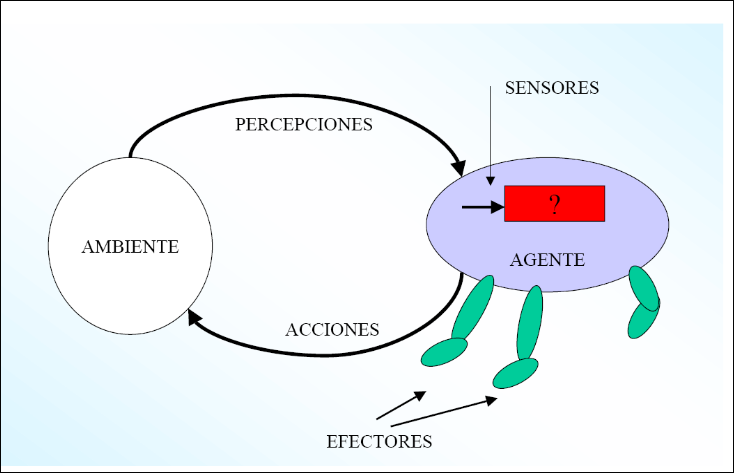
\includegraphics[width=0.5\textwidth]{images/Tema2/metodo.png}
    \caption{Método de reacción de un agente.}
    \label{fig:agentes}
\end{figure}

Ejemplo de estas percepciones, puede ser, para detectar el cáncer en alguna de las partes del cuerpo, se usan agentes que detectan la presencia de células cancerígenas en base a las imágenes del tumor.

Los agentes ofrecen una perspectiva innovadora
para representar la Inteligencia Artificial,
permitiendo abordar sus diversas áreas desde
un enfoque basado en agentes que ejecutan
acciones en función de percepciones procesadas
a través de mecanismos avanzados de análisis y
toma de decisiones.

Tema que cabe destacar, es que qen cuanto a la regulación de la IA, aún no esta decidida, si nos ponemos en el caso de que una IA causa algún daño, ¿quién es el responsable? ¿El creador de la IA o la IA en sí? Aún no se puede responder a esta pregunta.

Cuando tratamos el concepto de flecibilidad nos referimos a que sea capaz de realizar acciones de forma autónoma y que es
flexible para lograr los objetivos planteados.
\begin{itemize}
    \item Reactivo: reacciona en base al entorno.
    \item Pro-activo: no solo actúan en respuesta al entorno, sino que puedan analizar acciones a llevar a cabo.
    \item Social: son además capaces de interactuar con otros agentes.
\end{itemize}

Una \textit{nota imporatante} es el caso de GoogleMaps, ya que es deliberativo, pero esta diseño en cuanto a Software es reactivo.

Además, debemos de conocer el concepto de Sistema Multiagente, que es un sistema que se implementa como varios agentes interactuando entre sí, y de esta manera se consiguen numerosas versiones para resolver un problema.

Estos deben de ser capaces de cooperar, coordinarse y negociar entre ellos.

\subsection{IA Distribuida}

Destacamos los conceptos:
\begin{itemize}
    \item SMA: red más o menos unida de resolutores para solucionar problemas que solos sería más difícil.
    \item Resolutor: agente autónomo y de naturaleza heterogénea.
\end{itemize}

\subsubsection{Características}

Tiene información incompleta, no hay un sistema de control global, los datos no están centralizados y la computación es asincrónica.

\subsection{Arquitecturas de Agentes}

Podemos encontrarnos con las arquitecturas deliberativas y reactivas.

\subsubsection{Deliberativas}

Podemos encontrar un sistema de símbolso físicos, que es un conjunto de entidades físicas que pueden combinarse para formar estructuras más complejas. Se basa en la lógica y en la representación del conocimiento. Existe una \textit{hipótesis de sistema de símbolos inteligentes}, la cual dice qeu estos son capaces de generar acciones inteligentes.

Conocemos por \textit{Agente deliberativo} a  aquel que contiene un modelo simbólico del
mundo explícitamente representado, y cuyas decisiones se realizan a
través de un razonamiento lógico basado en emparejamientos de
patrones y manipulaciones simbólicas. Evalúa diferentes opciones de
acción considerando sus objetivos y selecciona la acción que
considera más adecuada según su razonamiento lógico.

Sabemos que toman decisiones en base a un razonamiento lógico, planificación y modelos internos del mundo.

Tenemos un problema: problema de representar simbólicamente la
información acerca de entidades y procesos
complejos del mundo real, y como conseguir que los
agentes razonen con esta información para que los
resultados sean útiles.

Como \textit{Ejemplo de agente deliberativo}, debemos de mencionar al problema del viajante del comercio, visto en otras Asignaturas como Algorítmica o Métodos Cuantitativos.
Este problema consiste en encontrar la ruta más corta que pasa por todas las ciudades y vuelve a la ciudad de origen.

\subsubsection{Reactivas}

Estos agentes reaccionan a la situación en la que se encuentran, eligiendo la acción más adecuada en base a lo que saben. No tienen un modelo interno del mundo, sino que reaccionan a la situación en la que se encuentran. Por lo que podemos decir que no hacen uso del razonamiento lógico.

\begin{figure}[H]
    \centering
    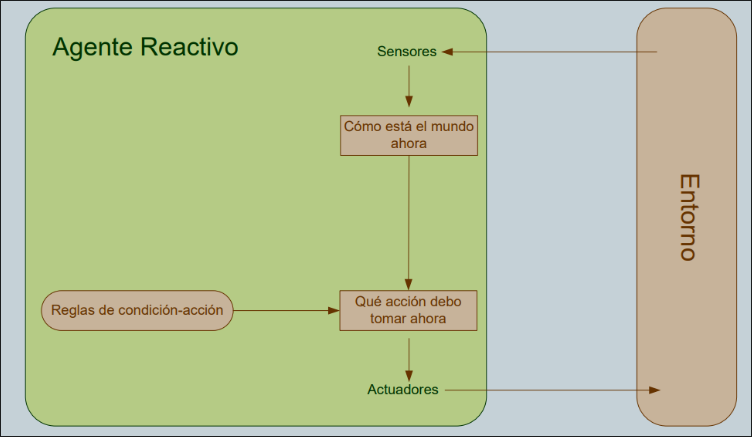
\includegraphics[width=0.7\textwidth]{images/Tema2/ar_re.png}
    \caption{Arquitectura reactiva.}
    \label{fig:reactivo}
\end{figure}

Uno de los ejemplos ed los agentes reactivos es \textit{es el robot que recorre un pasillo y evita obstáculos}. Este robot no tiene un modelo interno del mundo, sino que reacciona a la situación en la que se encuentra.

\subsubsection{Arquitecturas Híbridas}

Encontramos una estructura compuesta por capas reactivas y deliberativas. La capa reactiva se encarga de la percepción y la acción, mientras que la capa deliberativa se encarga de la planificación y el razonamiento. Tenemos una entrada sensorial, que se encarga de la percepción, y una salida motora, que se encarga de la acción.

Agente racional es similar a Agente inteligente.

En base a una serie de factores, podems definir un agente racional como: en cada posible secuencia de percepciones, un agente racional debe de seleccionar una acción que maximice su rendimiento, en base a la evidencia proporcionada por la secuencia de percepciones y en base al conocimiento que posee.

\subsection{Agentes Reactivos}

La característica principal de un agente reactivo es
su capacidad de responder directamente a estímulos
del entorno sin recurrir a un modelo interno o un
proceso de planificación. Este tipo de agente actúa
de manera inmediata basándose en reglas
predefinidas que relacionan percepciones con
acciones, lo que lo hace eficiente en entornos
dinámicos, aunque limitado en situaciones que
requieran razonamiento complejo.

En cuanto a las representaciones del mundo, podemos encontrar los módelos icónicos y los modelos basados en Características.

\subsubsection{Percepción y Acción}

El agente mediante estímulos a través de sensores, procesa la información, escoge una acción y la lleva a cabo mediante actuadores.

\begin{figure}[H]
    \centering
    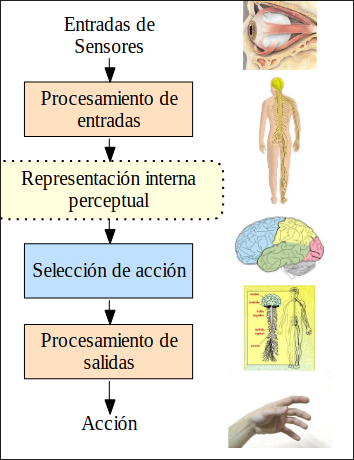
\includegraphics[width=0.4\textwidth]{images/Tema2/percep.png}
    \caption{Método de reacción de un agente.}
    \label{fig:agentes}
\end{figure}

\subsubsection*{Ejemplo del Diselo de un Agente Reactivo}
\begin{itemize}
    \item Ejemplo:
    \begin{itemize}
        \item Supongamos un robot en un mundo dividido en cuadrículas.
        \item El robot puede percibir si las 8 casillas vecinas están libres o no, con un sensor si por cada casilla i.
        \item El objetivo del robot es ir a una pared y seguir su perímetro indefinidamente.
        \item Tiene 4 posibles movimientos (de 1 casilla cada uno): Ir a Norte, Sur, Este u Oeste.
        \item No se permite que el entorno contenga pasillos estrechos (aquellas casillas rodeadas por dos o más obstáculos a ambos lados).
    \end{itemize}
\end{itemize}

Para verlo en detalle, ver las diapositivas 40-44.

\begin{itemize}
    \item Sistema de Producción: es un sistema de reglas que relacionan percepciones con acciones.
    \item Redes: son sistemas de reglas que se activan en paralelo.
    \item Arquitectura de subsunción: consiste en agrupar módulos de comportamiento en capas, donde cada capa tiene prioridad sobre la anterior. Cada módulo de comportamiento tiene una
    acción asociada, recibe la percepción
    directamente y comprueba una condición. Si esta
    se cumple, el módulo devuelve la acción a
    realizar.
    Un módulo se puede subsumir en otro. Si el
    módulo superior del esquema se cumple, se
    ejecuta este en lugar de los módulos inferiores.
\end{itemize}

\subsubsection{Agentes Reactivos con memoria}

Tiene ciertas limitaciones en cuanto al sistema sensorial, pero mejorar la precisión teniendo en cuenta la información previa.

Conocemos por \textit{Agente reactivo con memoria} a aquel que, además de reaccionar a la situación en la que se encuentra, tiene en cuenta información previa para mejorar la precisión de sus acciones.

Características de Agentes Reactivos:

\begin{itemize}
    \item Se diseñan completamente y por tanto es necesario anticipar todas
    las posibles reacciones para todas las situaciones.
    \item Realizan pocos cálculos y por tanto son rápidos.
    \item No tienen capacidad de aprendizaje.
    \item Almacenan todo en la memoria.
\end{itemize}

\begin{tcolorbox}[colback=yellow!10!white, colframe=yellow!90!black, title=¿Qué tipo de agente es ChatGPT?]
ChatGPT es un agente deliberativo, ya que utiliza un
proceso interno para generar respuestas basadas en
entradas del usuario, un vasto modelo de
conocimiento, y razonamiento complejo. Evalúa el
contexto y decide la mejor "acción" (respuesta) a
través de un procesamiento reflexivo y estructurado.
Sin embargo, también puede presentar características
reactivas, ya que responde rápidamente a estímulos
(mensajes) sin requerir planificación a largo plazo. Por
lo tanto, combina elementos deliberativos con un alto
grado de eficiencia reactiva. (Respuesta de Copilot).
\end{tcolorbox}

\begin{tcolorbox}[colback=red!10!white, colframe=red!90!black, title=Advertencia]
Solo es materia de examen las diapositivas que no tienen el título en rojo, que son las que tenemos todos los grados.
\end{tcolorbox}

% \chapter{Búsqueda en espacios de estados}
% \subsection{Diseño de un agente deliberativo: búsqueda en espacios de estados}

El agente dispone de un modelo del mundo donde actúa, modelo de efectos de las acciones sobre el mundo, es capaz de razonar sobre esos modelos para decidir que hacer para conseguir un objetivo.


Tras esta introducción, vamos a pasar a ver el espacio de estados.

\textbf{Espacio de Estados: } Representación del
conocimiento a través de las acciones del
agente.

\textbf{Búsqueda en Espacios de Estados: } Resolución del problema mediante proyección
de las distintas acciones.

Como ejemplo de agente deliberativo, se trata \textit{el problema del viajante de comercio}.

% Referencias
\newpage
% \begin{thebibliography}{99}
%   \bibitem{Referencia1} Ismael Sallami Moreno, \textbf{Estudiante del Doble Grado en Ingeniería Informática + ADE}, Universidad de Granada, 2025.
%   % \bibitem{Referencia2} Autor(es), \emph{Título del libro}, Editorial, año.
%   % \bibitem{Referencia3} Autor(es), \emph{Título del documento}, Nombre de la Conferencia, páginas, año.
% \end{thebibliography}

\begin{thebibliography}{99}
    \bibitem{russell} Stuart Russell y Peter Norvig, \textit{Artificial Intelligence: A Modern Approach}, 3rd Edition, Pearson, 2010.
    \bibitem{knuth} Donald E. Knuth y Ronald W. Moore, ``An Analysis of Alpha-Beta Pruning'', \textit{Artificial Intelligence}, 6(4), pp. 293–326, 1975.
    \bibitem{nash} Simon D. Nash, \textit{AI Game Programming Wisdom}, Charles River Media, 2002.
    \end{thebibliography}
    

\end{document}
